\section{Experimental Results}
\label{sec:results}

\begin{figure}[!t]
\centering
\subfloat[Performance Comparison]{
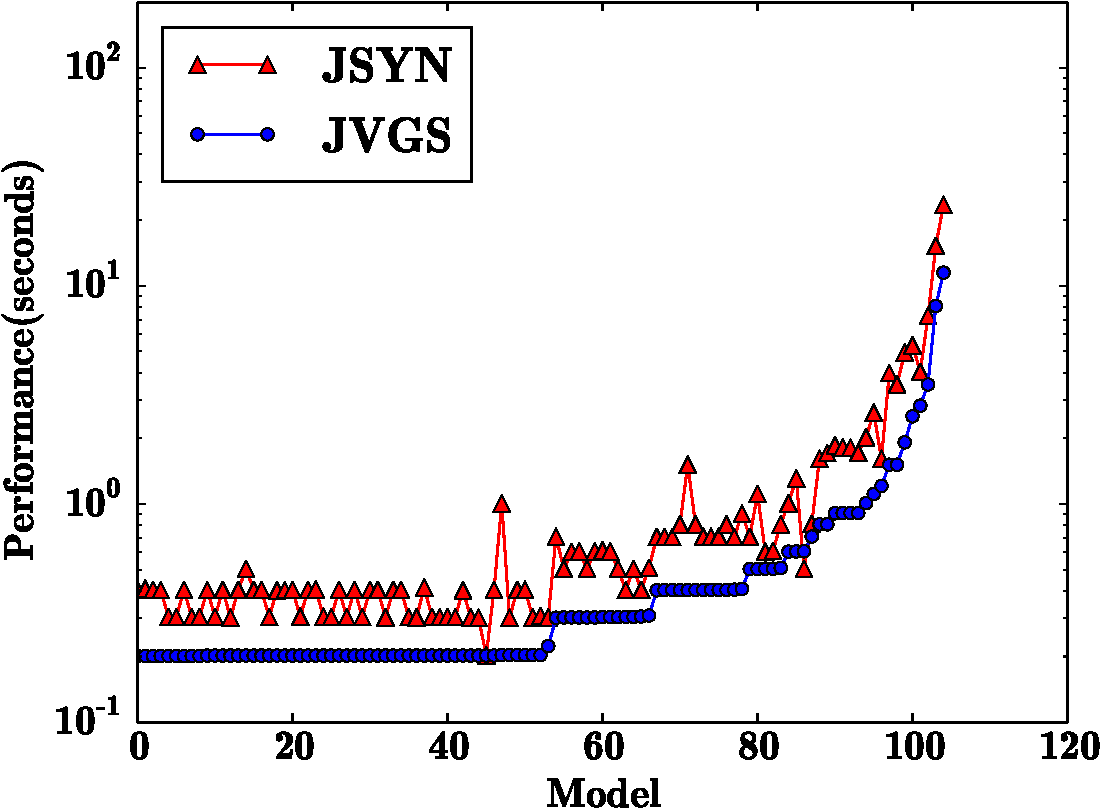
\includegraphics[width=2in]{overhead-crop}
\label{fg:performance}}
%\hspace{+6.5em}
\quad
\subfloat[Size of Synthesized
Implementations]{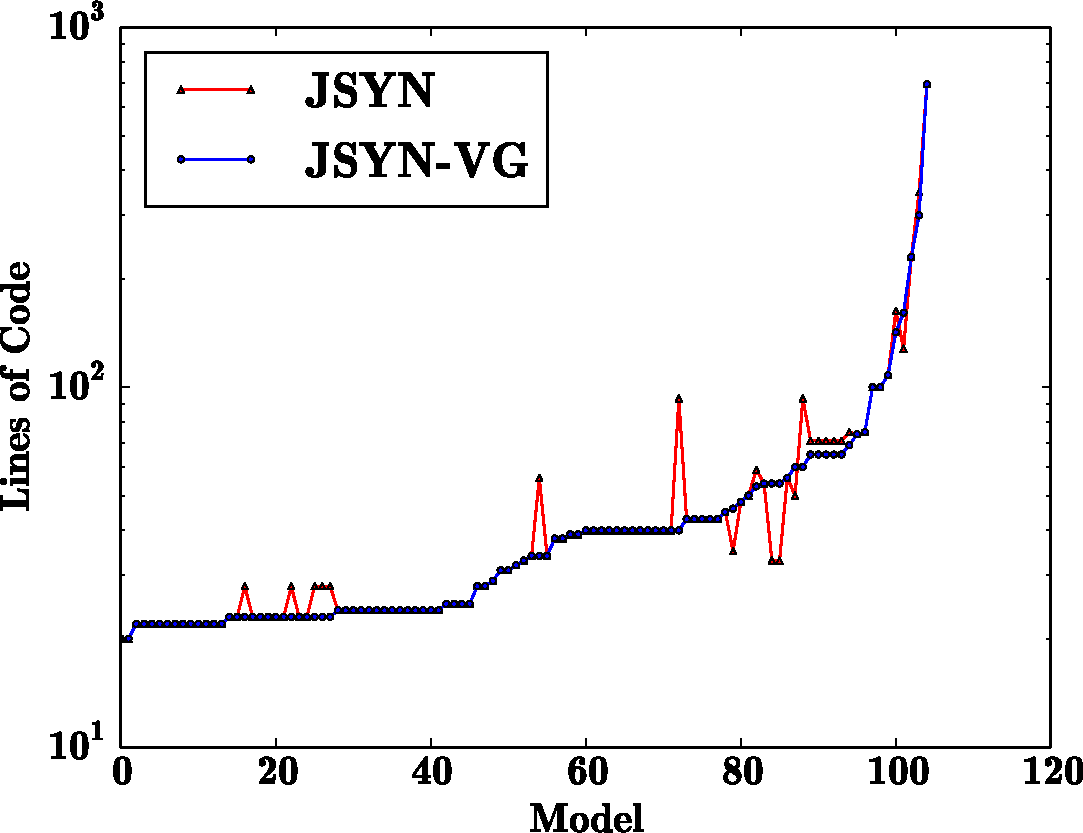
\includegraphics[width=2in]{loc-crop}
\label{fg:size}}
\quad
\subfloat[Performance of Synthesized Implementations]{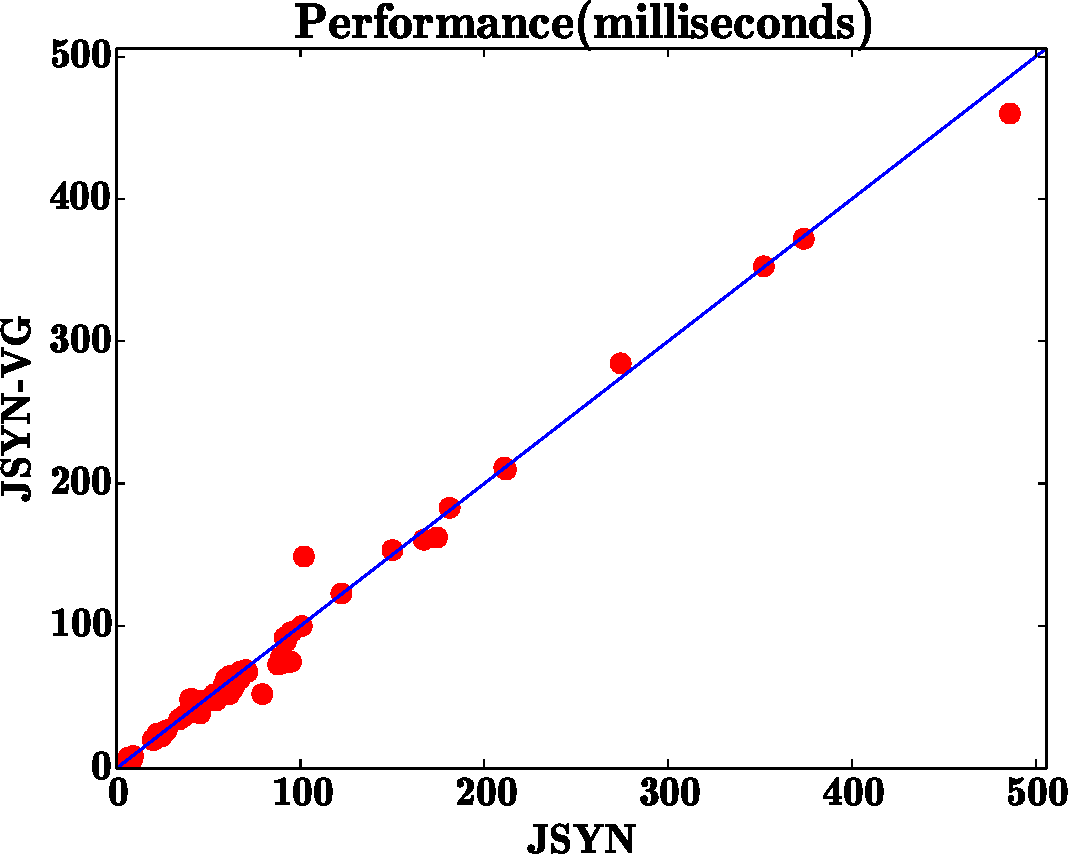
\includegraphics[width=2in]{performance-crop}
\label{fg:implperformance}}
\caption{Experimental results}
\label{fg:results}
\end{figure}

In this section we evaluate \jsynvg by synthesizing implementations
for 110 contracts that originate from a broad variety of contexts.~\footnote{An
anonymized repository containing the benchmark contracts can be found at
\url{https://tinyurl.com/mjtyxae }. We will replace this repository with the official for the camera-ready
version of the paper.} Almost half of them, 54, come from a collection of contracts that were initally used for the verification of existing handwritten implementations. The second biggest collection in our suite contains 46 contracts that correspond to various industrial projects, such as a Quad-Redundant Flight Control System, a Generic Patient Controlled Analgesia infusion pump, as well as a collection of contracts
for a Microwave model, written by graduate students as part of a software
engineering class. The remaining nine models contain variations of the
Cinderella-Stepmother game and the example in Section~\ref{sec:pre}.

The goal of this experiment was to determine the performance and generality of the \jsynvg algorithm.  We compared against the existing \jsyn algorithm, and for the Cinderella model, we compared against~\cite{beyene2014constraint} (this was the only synthesis problem in the paper).  We examined the following aspects: 
\begin{itemize}
    \item Time required to synthesize an implementation
    \item Size of generated implementations (in SLOC)
    \item Execution speed of generated C implementations derived from the synthesis procedure.
    \item Number of contracts that could be synthesized by each approach
\end{itemize}
\noindent Since \jkind already supports synthesis through \jsyn, we were able to directly
compare \jsynvg against \jsyn's k-inductive approach. We
ran the experiments using a computer with Intel Core i3-4010U 1.70GHz CPU and
16GB RAM.

\begin{table}[!t]
\centering
\caption{Benchmark Statistics}
\label{tbl:stats}
\resizebox{0.5\textwidth}{!}{%
\begin{tabular}{@{}lll@{}}
\toprule
 & \jsyn & \jsynvg \\ \midrule
Problems solved & 105 & \textbf{110} \\
Performance (avg - seconds) & 1.51 & \textbf{0.70} \\
Performance (max - seconds) & 26.06 & \textbf{12.85} \\
Implementation Size (avg - Lines of Code) & 51.15 & \textbf{49.74} \\
Implementation Size (max - Lines of Code) & 694 & 694 \\
Implementation Performance (avg - ms) & \textbf{58.83} & 60.91 \\
Implementation Performance (max - ms) & 466.195 & \textbf{406.109} \\
\bottomrule
\end{tabular}
}
\end{table}

\begin{table*}[!t]
\centering
\caption{Cinderella-Stepmother results}
\label{tbl:cindtbl}
\resizebox{\textwidth}{!}{%
\begin{tabular}{|c|c|c|c|c|c|}
\hline
\multirow{2}{*}{Game} & \multicolumn{3}{c|}{\jsynvg} & \multicolumn{2}{c|}{\textsc{ConSynth}~\cite{beyene2014constraint}} \\ \cline{2-6} 
 & Implementation Size (LoC) & Implementation Performance (ms) & Time & Time (Z3) & Time (Barcelogic) \\ \hline
Cinderella (C = 3) & 92 & 262.84 & 35s & \multirow{2}{*}{3.2s} & \multirow{2}{*}{1.2s} \\ \cline{1-4}
Cinderella2 (C = 3) & 222 & 309.24 & 2m9s &  &  \\ \hline
Cinderella (C = 2) & 102 & 196.57 & 24s & \multirow{2}{*}{1m52s} & \multirow{2}{*}{1m52s} \\ \cline{1-4}
Cinderella2 (C = 2) & 272 & 230.16 & 2m9s &  &  \\ \hline
\end{tabular}}
\end{table*}
% \begin{table*}[!t]
% \centering
% \caption{Cinderella-Stepmother results}
% \label{tbl:cindtbl}
% \begin{tabular}{|c|c|c|c|c|c|}
% \hline
%  & \multicolumn{3}{c|}{\jsynvg} & \multicolumn{2}{c|}{\textsc{ConSynth}~\cite{beyene2014constraint}} \\ \hline
%  & Implementation Size (LoC) & Implementation Performance (ms) & Time & Time (Z3) & Time (Barcelogic) \\ \hline
% Cinderella (C = 3) & 92 & 262.84 & 35s & \multirow{2}{*}{3.2s} & \multirow{2}{*}{1.2s} \\ \cline{1-4}
% Cinderella2 (C = 3) & 222 & 309.24 & 2m9s &  &  \\ \hline
% Cinderella (C = 2) & 102 & 196.57 & 24s & \multirow{2}{*}{1m52s} & \multirow{2}{*}{1m52s} \\ \cline{1-4}
% Cinderella2 (C = 2) & 272 & 230.16 & 2m9s &  &  \\ \hline
% \end{tabular}
% \end{table*}

A listing of the statistics that we tracked while running experiments is
presented in Table~\ref{tbl:stats}.
Figure~\ref{fg:performance} shows the time allocated by \jsyn and \jsynvg to solve each problem, with \jsynvg
outperforming \jsyn across the board, often times by a margin greater than
50\%. Figure~\ref{fg:size} on the other hand, depicts small differences in the
overall size between the synthesized implementations. While it would be
reasonable to conclude that there are no noticable improvements, the bigger
picture is different. The key factor that is not apparent from this figure, is the length of the k-inductive proof. For the majority of the benchmarks in the suite, \jsyn proves their realizability by constructing proofs of length $k=0$, which essentially means
that the entire space of states is an inductive invariant. As such, \jsynvg
also manages to synthesize implementations without requiring any refinement
process. For these cases, both algorithms generate a single Skolem function. In the general case though, the size of \jsyn solutions is directly
dependent on $k$, since each implementation is composed of $k$ Skolem
functions ($k-1$ to initialize the system, and one last for the inductive step),
where the equivalent solution from \jsynvg is always just one.
Figure~\ref{fg:size} hints towards this intuition, through a handful of spikes
in \jsyn implementation size. Despite this, we also noticed cases where \jsyn
implementations are shorter. This provides us with another interesting
observation regarding the formulation of the problem for $k=0$ proofs. In
these cases, \jsyn proves the existence of viable states, starting from a set
of \textit{pre-initial} states, where the contract does not need to hold. This
has direct implications to the way that the $\forall\exists$-formulas are
constructed in \jsyn's underlying machinery, where the assumptions are ``baked''
into the transition relation, affecting thus the creation of Model-Based
Projections by \aeval.

 One last statistic that we tracked was the performance of the synthesized C
 implementations, which can be seen in Figure~\ref{fg:implperformance}. For this purpose, we translated the
 generated witnesses from \jsyn and \jsynvg solutions using
 \smtlibtoc under the same set of options. Table~\ref{tbl:stats} shows that
 while \jsyn implementations are faster, the difference is minuscule on average.
This may be in part because \jsyn creates separate skolem functions for the initial evaluation (when \%init is true) and subsequent evaluations, whereas currently \jsynvg uses a single function for both the initial and subsequent steps.  We are considering specialization of the generated \jsynvg functions based on \%init, as well as several other optimizations of the generated code in future work.


% The deciding factor in this context is the
% difference in complexity of the Model-Based Projections that get generated by
% \aeval using \jsyn and \jsynvg, with the latter versions containing richer
% expressions, mainly due to the refinement process.

Figure~\ref{fg:results} does not cover the entirety of the
benchmark suite. From the original 110 problems, five of them cannot be
solved by \jsyn's k-inductive approach. Four of these files are variations of
the cinderella-stepmother game that we described in Section~\ref{sec:example}, using different representations of the game, as well as two different values
for the bucket capacity (2 and 3). Using the variation that we included in the
aforementioned section as an input to \jsyn, we receive an ``unrealizable'' answer, with the counterexample shown
in Figure~\ref{fg:cex}. Reading through the feedback provided by \jsyn, it is
apparent that the underlying SMT solver is incapable of choosing the correct
buckets to empty, leading eventually to a state where an overflow occurs for the
third bucket. As we already discussed though, a winning strategy exists for the
cinderella, as long as the bucket capacity $c$ is between 1.5 and 3. This
provides an excellent demonstration regarding the inherent weakness of \jsyn
in providing sound ``unrealizable'' results. \jsynvg's validity-guided approach,
on the other hand, was able to prove the realizability for these contracts, as
well as synthesize an implementation for each.

\begin{figure}[!t]
 \begin{Verbatim}[fontsize=\tiny]
			 ++++++++++++++++++++++++++++++++++++++++++++++++++++++++++
			      UNREALIZABLE || K = 6 || Time = 2.017s
			                 Step
			      variable      0    1      2      3      4      5
			      INPUTS
			      i1            0    0      0 0.416* 0.944* 0.666*
			      i2            1    0 0.083* 0.083*      0 0.055*
			      i3            0    1 0.305*    0.5 0.027* 0.194*
			      i4            0    0 0.611*      0      0 0.027*
			      i5            0    0      0      0 0.027* 0.055*
			
			      OUTPUTS
			      e             1    3      1      5      4      5
			
			      NODE OUTPUTS
			      guarantee   true true   true   true   true  false
			
			      NODE LOCALS
			      b1            0    0      0 0.416* 1.361* 0.666*
			      b2            0    0 0.083* 0.166* 0.166* 0.222*
			      b3            0    1 1.305* 1.805* 1.833* 2.027*
			      b4            0    0 0.611* 0.611*      0 0.027*
			      b5            0    0      0      0 0.027* 0.055*
			
			      * display value has been truncated
			 ++++++++++++++++++++++++++++++++++++++++++++++++++++++++++
 \end{Verbatim}
\caption{Spurious counterexample for Cinderella-Stepmother example using \jsyn}

\label{fg:cex}
\end{figure}

Table~\ref{tbl:cindtbl} shows how \jsynvg performed against the four contracts describing the Cinderella-Stepmother game. We used two different interpretations for the game, and exercised both for the cases where the bucket capacity $C$ is equal to 2 and 3. The performance is heavily affected when we exercise the variation for $C=2$, but \jsynvg is still able to synthesize a winning region for Cinderella. Regarding the synthesized implementations, their size remains analogous to the difficulty of the problem, in conjunction with the complexity of the program (Cinderella2 contains more local variables and a helper function to empty buckets). Despite this, the implementation performance remains at the same levels across all implementations. Finally for reference, the table contains the results from the template-based approach followed in \textsc{Consynth}~\cite{beyene2014constraint}. From the results, it is apparent that providing templates dramatically increases the performance of the underlying synthesis procedure. Nevertheless, the automated approach in \jsynvg is able to synthesize solutions for the same problems in a reasonable time margin, when compared to \textsc{ConSynth}.


Overall, \jsynvg's validity-guided approach provides significant advantages
over the k-inductive technique followed in \jsyn, and effectively expands
\jkind's solving capabilities regarding specification realizability. On top of that, it provides an efficient ``hands-off'' approach that is capable of solving complex games.
The most significant contribution, however, is the applicability of this approach, as it is not tied to a specific environment since it can be extended to support more
theories, as well as categories of specification.
